%----------------------------------------------------------------------------------------
%	PACKAGES AND OTHER DOCUMENT CONFIGURATIONS
%----------------------------------------------------------------------------------------

\documentclass[
	10pt, % Set the default font size, options include: 8pt, 9pt, 10pt, 11pt, 12pt, 14pt, 17pt, 20pt
	%t, % Uncomment to vertically align all slide content to the top of the slide, rather than the default centered
	%aspectratio=169, % Uncomment to set the aspect ratio to a 16:9 ratio which matches the aspect ratio of 1080p and 4K screens and projectors
	hmargin=1cm,vmargin=0cm,head=0.5cm,headsep=0pt,foot=0.5cm,margin=2cm
]{beamer}

% Hide navigation symbols
\setbeamertemplate{navigation symbols}{}
 
\usepackage{caption}
\captionsetup{labelformat=empty,labelsep=none}
\graphicspath{{images/}{./}} % Specifies where to look for included images (trailing slash required)
\usepackage{minted}
\usepackage{amsmath}
\usepackage{multirow}
\usepackage{color, colortbl}
\usepackage{xcolor}
\usepackage{booktabs} % Allows the use of \toprule, \midrule and \bottomrule for better rules in tables
\usepackage{graphicx}
\usepackage{minibox}
\renewcommand{\arraystretch}{1.2} % Default value: 1
\definecolor{darkGreen}{RGB}{9,150,3} 
\usepackage{tikz}

\newcommand{\tikzunderarrow}[2][black]{\tikz[baseline={(N.base)}]{
  \node[inner sep=0, outer sep=0](N) {#2};
  \draw[overlay, -latex, line width=.04em, #1]
    ([yshift=-.14em]N.south west) -- ([yshift=-.14em]N.south east);}}
\usepackage{ragged2e}
\tolerance=1
\emergencystretch=\maxdimen
\hyphenpenalty=10000
\hbadness=10000

%	SELECT LAYOUT THEME
%----------------------------------------------------------------------------------------
%
% Beamer comes with a number of default layout themes which change the colors and layouts of slides. Below is a list of all themes available, uncomment each in turn to see what they look like.

%\usetheme{default}
%\usetheme{AnnArbor}
%\usetheme{Antibes}
%\usetheme{Bergen}
%\usetheme{Berkeley}
% \usetheme{Berlin}
%\usetheme{Boadilla}
% \usetheme{CambridgeUS}
% \usetheme{Copenhagen}
% \usetheme{Darmstadt}
% \usetheme{Dresden}
% \usetheme{Frankfurt}
% \usetheme{Goettingen}
% \usetheme{Hannover}
% \usetheme{Ilmenau}
% \usetheme{JuanLesPins}
% \usetheme{Luebeck}
\usetheme{Madrid}
%\usetheme{Malmoe}
%\usetheme{Marburg}
%\usetheme{Montpellier}
%\usetheme{PaloAlto}
%\usetheme{Pittsburgh}
%\usetheme{Rochester}
%\usetheme{Singapore}
%\usetheme{Szeged}
%\usetheme{Warsaw}

%----------------------------------------------------------------------------------------
%	SELECT COLOR THEME
%----------------------------------------------------------------------------------------

% Beamer comes with a number of color themes that can be applied to any layout theme to change its colors. Uncomment each of these in turn to see how they change the colors of your selected layout theme.

% \usecolortheme{albatross}
% \usecolortheme{beaver}
% \usecolortheme{beetle}
% \usecolortheme{crane}
% \usecolortheme{dolphin}
% \usecolortheme{dove}
% \usecolortheme{fly}
% \usecolortheme{lily}
% \usecolortheme{monarca}
% \usecolortheme{seagull}
% \usecolortheme{seahorse}
\usecolortheme{spruce}
% \usecolortheme{whale}
% \usecolortheme{wolverine}

%----------------------------------------------------------------------------------------
%	SELECT FONT THEME & FONTS
%----------------------------------------------------------------------------------------

% Beamer comes with several font themes to easily change the fonts used in various parts of the presentation. Review the comments beside each one to decide if you would like to use it. Note that additional options can be specified for several of these font themes, consult the beamer documentation for more information.

\usefonttheme{default} % Typeset using the default sans serif font
%\usefonttheme{serif} % Typeset using the default serif font (make sure a sans font isn't being set as the default font if you use this option!)
\usefonttheme{structurebold} % Typeset important structure text (titles, headlines, footlines, sidebar, etc) in bold
%\usefonttheme{structureitalicserif} % Typeset important structure text (titles, headlines, footlines, sidebar, etc) in italic serif
%\usefonttheme{structuresmallcapsserif} % Typeset important structure text (titles, headlines, footlines, sidebar, etc) in small caps serif

%------------------------------------------------

%\usepackage{mathptmx} % Use the Times font for serif text
\usepackage{palatino} % Use the Palatino font for serif text

%\usepackage{helvet} % Use the Helvetica font for sans serif text
\usepackage[default]{opensans} % Use the Open Sans font for sans serif text
%\usepackage[default]{FiraSans} % Use the Fira Sans font for sans serif text
%\usepackage[default]{lato} % Use the Lato font for sans serif text

%----------------------------------------------------------------------------------------
%	SELECT INNER THEME
%----------------------------------------------------------------------------------------

% Inner themes change the styling of internal slide elements, for example: bullet points, blocks, bibliography entries, title pages, theorems, etc. Uncomment each theme in turn to see what changes it makes to your presentation.

%\useinnertheme{default}
\useinnertheme{circles}
% \useinnertheme{rectangles}
% \useinnertheme{rounded}
%\useinnertheme{inmargin}

%----------------------------------------------------------------------------------------
%	SELECT OUTER THEME
%----------------------------------------------------------------------------------------

% Outer themes change the overall layout of slides, such as: header and footer lines, sidebars and slide titles. Uncomment each theme in turn to see what changes it makes to your presentation.

% \useoutertheme{default}
% \useoutertheme{infolines}
\useoutertheme{miniframes}
% \useoutertheme{smoothbars}
% \useoutertheme{sidebar}
%\useoutertheme{split}
% \useoutertheme{shadow}
% \useoutertheme{tree}
%\useoutertheme{smoothtree}
%----------------------------------------------------------------------------------------
%	PRESENTATION INFORMATION
%----------------------------------------------------------------------------------------

\title[LAB 05: Arrays and Files]{LAB 05: Arrays and Files} % The short title in the optional parameter appears at the bottom of every slide, the full title in the main parameter is only on the title page

\author[S. AlSaleh]{Saleh AlSaleh \\ \smallskip \textit{salehs@kfupm.edu.sa}} % Presenter name(s), the optional parameter can contain a shortened version to appear on the bottom of every slide, while the main parameter will appear on the title slide

\institute[KFUPM]{King Fahd University of Petroleum and Minerals \\ College of Computing and Mathematics \\ Computer Engineering Department} % Your institution, the optional parameter can be used for the institution shorthand and will appear on the bottom of every slide after author names, while the required parameter is used on the title slide and can include your email address or additional information on separate lines

\date[February 12, 2023]{COE301: Computer Architecture \\ Term 222} % Presentation date or conference/meeting name, the optional parameter can contain a shortened version to appear on the bottom of every slide, while the required parameter value is output to the title slide

%----------------------------------------------------------------------------------------

\begin{document}

%----------------------------------------------------------------------------------------
%	TITLE SLIDE
%----------------------------------------------------------------------------------------

\begin{frame}
	% Output the title slide, automatically created using the text entered in the PRESENTATION INFORMATION block above
	\titlepage
\end{frame}

%----------------------------------------------------------------------------------------
%	TABLE OF CONTENTS SLIDE
%----------------------------------------------------------------------------------------

\begin{frame}
	\frametitle{Agenda} % Slide title, remove this command for no title
	\tableofcontents % Output the table of contents (all sections on one slide)
\end{frame}

%----------------------------------------------------------------------------------------
%	PRESENTATION BODY SLIDES
%----------------------------------------------------------------------------------------

\section{Static Allocation} 
\begin{frame}
	\frametitle{Static Allocation}
	
	\begin{itemize}
		\item Allocates one variable or an array of variables in the static area of data segment. \pause
		\item Array size is determined at assemble time. \pause
		\item Data types: byte (8 bits), half-word (16 bits), word (32 bits). \pause
		\item Declaration and initialization at the same time example:
		\begin{columns}[c]
			\begin{column}{0.45\textwidth}
				\color{red}.data \color{black} \\
				secretbyte: \hspace{.2cm}\color{red}.byte\color{black}\hspace{.33cm} 0xAB \\ 
				secrethalf: \hspace{.30cm}\color{red}.half\color{black}\hspace{.45cm} 0xABCD \\ 
				secretword: \hspace{.065cm}\color{red}.word\color{black}\hspace{.22cm} 0x89ABCDEF \\ 
				\pause
			\end{column}
			\begin{column}{0.45\textwidth}
				\color{red}.data \color{black} \\ 
				secretbytes: \hspace{.18cm}\color{red}.byte\color{black}\hspace{.1cm}  0xAB:10 \\ 
				secrethalves: \hspace{.02cm}\color{red}.half\color{black}\hspace{.82cm}    0:15 \\ 
				secretwords: \hspace{.05cm}\color{red}.word\color{black}\hspace{.6cm}     1:20 \\
				\pause
			\end{column}
		\end{columns}
		\item Declaration only example: \\
			\color{red}.data \color{black} \\ 
			secretarr: \color{red}.space\color{black}\hspace{.1cm} 100
	\end{itemize}
\end{frame}

\section{Dynamic Allocation} 
\begin{frame}
	\frametitle{Dynamic Allocation}
	\begin{itemize}
		\item Allocates one or more bytes at run time in the dynamic area (heap) of the data segment.\pause
		\item Some programs require different array sizes based on some inputs. \pause
		\item Use system call (\color{red}\$v0\color{black}\hspace{0.05cm} = 9) and number of bytes to allocate in \color{red}\$a0\color{black}. \pause
		\item The base address will be returned in \color{red}\$v0\color{black}, this base address needs to be saved. \pause
		\item Example: \\
		\color{blue}li \color{red}\$v0\color{black}, 9 \\
		\color{blue}li \color{red}\$a0\color{black}, 30 \\ 
		\color{blue}syscall \color{black} \\ 
		\# base address will be stored in \$v0 \\ 
	\end{itemize}
\end{frame}

\section{Memory Organization}
\begin{frame}
	\frametitle{Memory Organization}
	\begin{figure}
		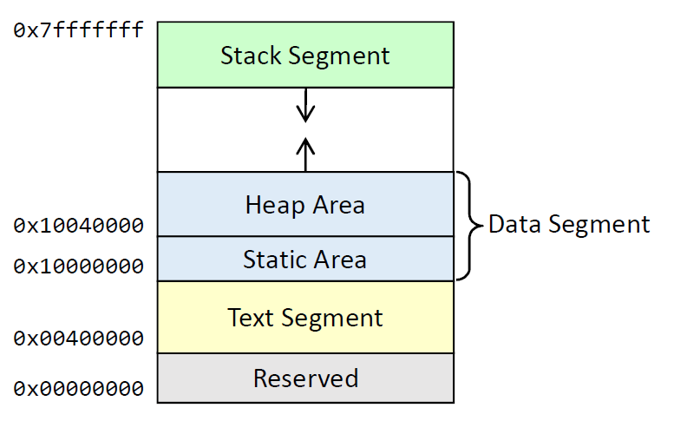
\includegraphics[width=0.5\linewidth]{mips_memory.png}
		\caption{MIPS Memory Organization}
	\end{figure}
\end{frame}

\section{Address Calculation}
\begin{frame}
	\frametitle{Address Calculation}
	\begin{itemize}
		\item 1-D Array Address Calculation
		\begin{itemize}
			\item arr1D: .type 0:20 \# e.g. int arr1D[20]; \pause
			\item Address of arr1D[i] =  \\ \pause
			\hspace{2cm} base\_address(arr1D) + (i * element\_size) \pause
		\end{itemize}
		\item 2-D Array Address Calculation
		\begin{itemize}
			\item arr2D: .type 0:20 \# e.g. int arr1D[4][5]; \pause
			\item Address of arr2D[i][j] = \\ \pause
			\hspace{0.2cm} base\_address(arr2D) + (i * col\_size * element\_size) + (j * element\_size)
		\end{itemize}
	\end{itemize}
\end{frame}


\section{Files}
\begin{frame}
	\frametitle{Files}
	\begin{itemize}
		\item They provide an easy method to test applications that require many input and output values. \pause
		\item For a file to be used, it needs to be \textbf{opened FIRST}. \pause
		\item System Call \textbf{13} is used to open a file with the following options:
			\begin{itemize}
			\item \color{red}\$a0\color{black}\hspace{.05cm} address of null-terminated string containing the file name. \\
			Path can be relative to the location of MARS.jar file or an absolute path.
			\item \color{red}\$a1\color{black}\hspace{.05cm} = 0 for read-only.
			\item \color{red}\$a1\color{black}\hspace{.05cm} = 1 for write-only with truncate and create.
			\item \color{red}\$a1\color{black}\hspace{.05cm} = 9 for write-only with create and append.
			\end{itemize}
		\item It returns in \color{red}\$v0\color{black}\hspace{.05cm} a positive file descriptor if it can open the file or negative if error.
		\item File descriptor \textbf{NEEDS} to be saved for other system calls.
	\end{itemize}
\end{frame}
\begin{frame}
	\frametitle{Files}
	\begin{itemize}
		\item System Call \textbf{14} is used to read file contents with the following options:
		\begin{itemize}
			\item  \color{red}\$a0 \color{black}\hspace{0.05cm} = file descriptor 
			\item  \color{red}\$a1 \color{black}\hspace{0.05cm} = address of input buffer
			\item  \color{red}\$a2 \color{black}\hspace{0.05cm} = maximum number of characters to read
		\end{itemize}
		\item It returns in \color{red}\$v0\color{black}\hspace{0.05cm} a positive number of characters read, zero if end of file or negative if error. \pause
		\item System Call \textbf{15} is used to write contents to file with the following options:
		\begin{itemize}
			\item \color{red}\$a0\color{black}\hspace{0.05cm} = file descriptor 
			\item \color{red}\$a1\color{black}\hspace{0.05cm} = address of output buffer
			\item \color{red}\$a2\color{black}\hspace{0.05cm} = number of characters to write
		\end{itemize}
		\item It returns in \color{red}\$v0\color{black}\hspace{0.05cm} a positive number of characters written or negative if error. \pause
		\item System Call \textbf{16} is used to close file with \color{red}\$a0\color{black}\hspace{0.05cm} containing the file descriptor.
	\end{itemize}
\end{frame}

\section{Live Examples}
\begin{frame}
	\frametitle{Live Examples}
	
\end{frame}

%------------------------------------------------

\section{Tasks}

\begin{frame}[fragile]
	\frametitle{Task \#1}
	\begin{columns}[c]
		\begin{column}{0.55\textwidth}
		
			\justifying
			Write a MIPS assembly program that reads the size (n) of the message from the user. Then, the program allocates (n+1) bytes in the heap. After that, read a string of n characters from the user he/she wishes to encrypt. Next, read an encrypting key (e) from the user [1, 25]. Encrypt the original string with the encryption key using the following code. Finally, print out the encrypted string.

			\centering
			Sample Run

			\minibox[frame,pad=4pt]{
				\color{black} Enter n: \color{blue} 11 \\
				\color{black} Enter string: \color{blue} Hello World \\
				\color{black} Enter e: \color{blue} 13 \\
				\color{black} Encrypted string = \color{darkGreen} Uryyb Jbeyq \\
			}	
		\end{column}
		\begin{column}{0.45\textwidth}
		\begin{listing}[H]
			\centering			
			\begin{minted}[frame=single,autogobble,xleftmargin=0.1\textwidth,xrightmargin=0.1\textwidth,framesep=2mm,baselinestretch=1.2,fontsize=\footnotesize,obeytabs,tabsize=2]{c}
			for(i=0;i<n;i++){
				ch = str[i];
				if(isupper(ch)){
					ch = ch + e;
					if (ch > 0x5A)
						ch = ch - 26;
					}
				else if(islower(ch)){
					ch = ch + e;
					if (ch > 0x7A)
						ch = ch - 26;
					}
				str[i] = ch;
			}
			\end{minted}
			\caption{Caesar Encryption Algorithm}
			\end{listing}
		\end{column}
	\end{columns}
\end{frame}

\begin{frame}
	\frametitle{Task \#2}
	\begin{columns}[c]
		\begin{column}{0.6\textwidth}
			\justifying
			Write a MIPS assembly program that asks the user for file name (max 50 chars). Open the file for reading. Next, read the file contents as characters (max 100 chars). After that, loop over each character, if the character is a digit (i.e. `0' to `9'), convert it to integer and store it in another array called ``array\_int''. Assume the maximum number of integers in the file is 20. Finally, print ``array\_int'' in reverse order. \\
			
			
			\vspace{0.3cm}
			\centering
			Sample Run 

			\minibox[frame,pad=4pt]{
				\color{black}Enter filename: \color{blue}numbers.txt \\
				\color{black}Integer array reversed = \color{darkGreen}1 5 8 9 7 6 5 4 3 2 1 \\
			}
		\end{column}
		\begin{column}{0.4\textwidth}
		\centering
			Static data segment 

			\minibox[frame,pad=4pt]{
				.data \\
				filename: .space 50 \\
				filecontents: .space 100 \\
				array\_int: .word 0:20 \\
			}
			\vspace{0.5cm}
			
			Sample File (numbers.txt)

			\minibox[frame,pad=4pt]{
				1 2 3 4 5 6 \\
				7 9 hello, world \\
				851 \\
			}
			
			
		\end{column}
	\end{columns}
\end{frame}

%----------------------------------------------------------------------------------------

\end{document} 
